%!TEX root = main.tex
\chapter{Design}
In this chapter the design process will be explained in detail. We will show how our tool went from sketch to a full live web-page. 
Through the different iterations of development, we made different design choices that helped design the application. Before the actual development began, we went
through a design process that resulted in a basis for implementation. In this section we will elaborate on how these steps culminated into the final design choice.
\section{Responsive web design}
Responsive web design\cite{responsivearticle} is a web design approach aimed at developing websites in order to provide an optimal viewing experience on a wide range of devices, from large desktop monitors to smartphones and tablets. This includes easy reading and navigation with minimal resizing, panning, and scrolling.\\
Any site designed to be responsive, adapts the layout to the viewing environment, along with fluid proportion-based grids and flexible images.\\
\begin{figure}[h!]
\label{responsivelayout}
\centering
	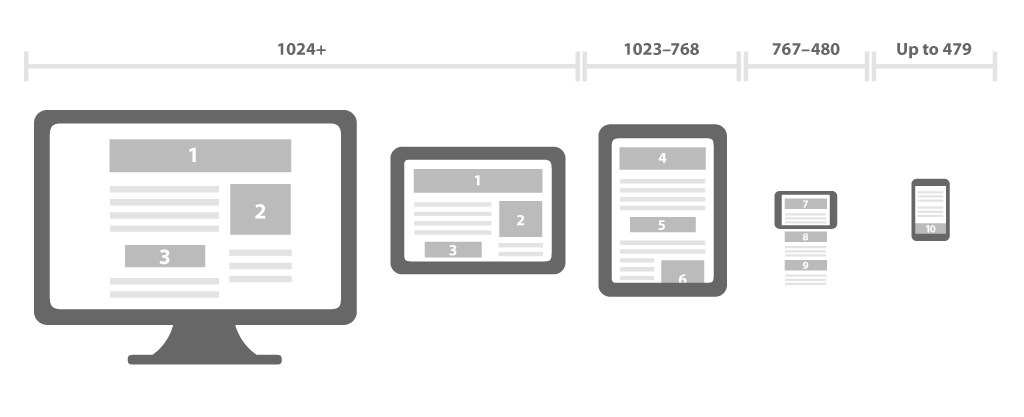
\includegraphics[width=\textwidth]{responsivelayout}
\caption{Responsive layout, adapting the same content to different viewing experiences}
\end{figure}

\subsection{Fluid grid}
A definition on fluid is : ``A fluid is a substance that continually deforms (flows) under an applied shear stress''\cite{fluidgrid}. In a web-design context, fluid will be the design and layout, and shear stress will be the device used to access the content.
Regardless of what the device or screen size is, components in fluid designs are going to flow and adapt to the user environment. Fluid grids define a maximum layout size and the grid is divided into columns for easier handling. These grids can then be designed with proportional widths and heights. The fluid grid and it's columns can be seen in Figure \ref{responsivelayout}.
The fluid grid\cite{fluidgrid, fluidarticle} concept states that page elements should be sized in relative units, like percentages or ems, instead of absolute units like pixels or points. Since fluid grids flow naturally based on the dimensions of its parent container-component, specific adjustments for various devices are therefore kept to a minimum. In the fluid grid, flexible images are also sized in relative units, up to 100\%, in order to prevent them from stretching outside their containing element\cite{fluidimages}. This means all kinds of elements on a web-page can be treated as proportions measured against their container, and not in absolute pixels. 

\section{Mockups}
At the very beginning we had an idea of what we wanted to do and how to do it. At the time we had not decided on a platform for our application. Because of this we sketched up some different design choices.

\subsection{Smartphone App}
Our first alternative was creating a native app for smartphones, on iOS or Android. We had experience with creating android applications before, so this was our first thought. 
\begin{figure}[h!]
\label{smartphonemock}
\centering
	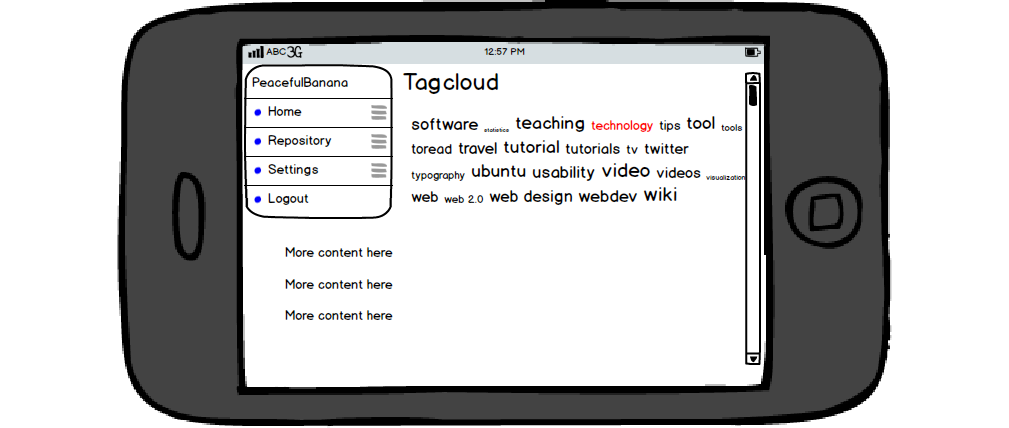
\includegraphics[width=\textwidth]{smartphonemock}
\caption{Smartphone mockup}
\end{figure}

\subsection{Web-Application tool}
Our second option was creating our tool as a web-application. Web-applications are platform independant and can be accessed on a wide range of devices, as long as it has a fairly updated browser. The idea was to also make the web application responsive, which would provide an optimized viewing experience allowing for easy reading and navigation with minimal resizing, panning, and scrolling—across a wide range of devices (from large monitors to mobile phones .\\
This is how our first sketch for a web-app looked like: 
\begin{figure}[h!]
\label{webappmock}
\centering 
	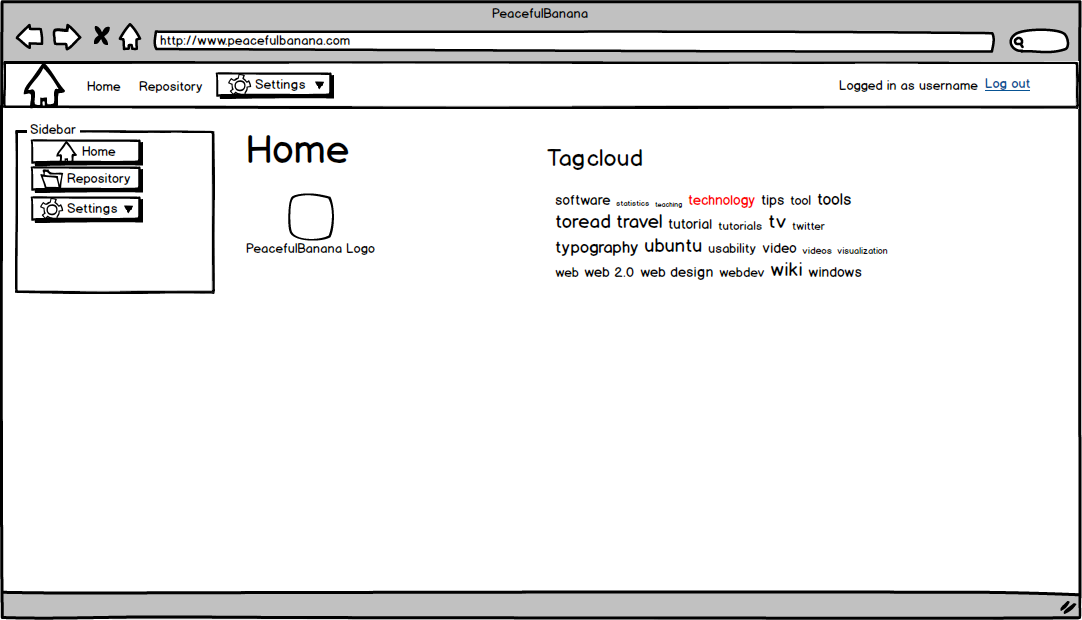
\includegraphics[width=\textwidth]{webappmock}
\caption{Web-app mockup}
\end{figure}
As this was the main design options, we did some research on existing frameworks which might suit our requirements. The tool needed to be responsive and work on a wide range of devices, which made a fluid design suitable.

\section{Twitter Bootstrap}
The Twitter Bootstrap framework\cite{twitterbootstrap} features exactly the requirements stated above. Bootstrap was developed by Mark Otto and Jacob Thornton at Twitter, as a framework to promote consistency in internal tools\cite{buildingbootstrap}. Twitter bootstrap is a free powerful front-end framework for faster and easier web development, and it's publically available to use by anyone.\\ It contains HTML and CSS based design templates for interface elements like buttons, charts, and navigation. Bootstrap was made to to not only look and behave optimally in desktop browsers, but in tablet and smartphone browsers via responsive CSS and HTML5 as well. The framework features responsive grids, components like tabs and dropdowns, JavaScript plugins, typography options and forms. \\
Twitter Bootstrap is the most popular project in GitHub and is used by amongst others NASA(National Aeronautics and Space Administration)\cite{nasa}
Bootstrap is also modular, which means it is composed of a series of components that together make the toolkit. Developers can then cherry pick the components they need from the Bootstrap toolkit. \\

\subsection{Bootstrap grid}
Bootstrap ships with the standard 940 pixel wide, grid layout. Developers can choose to use a variable-width layout if they wish. In any case the Bootstrap toolkit has four major variations in order to adapt content and grid width to different resolutions and devices: mobile phones, both portrait and landscape format, tablets and desktop computers with both low and high resolution/widescreen support.

\subsection{Bootstrap components}
Bootstrap features a set of CSS stylesheet, which defines styles for the major HTML elements. These stylesheets allow for a platform-independent, multibrowser enabled and consistent appearance for text, tables and other elements. \\
Bootstrap also comes with additional commonly used interface components. Such components are buttons, button-groups, buttons with drop-down option, navigation lists, tabs, breadcrumbs, pagination, different alerts and so on. 
\begin{figure}[h!]
\label{bootstrapbutton}
\centering
	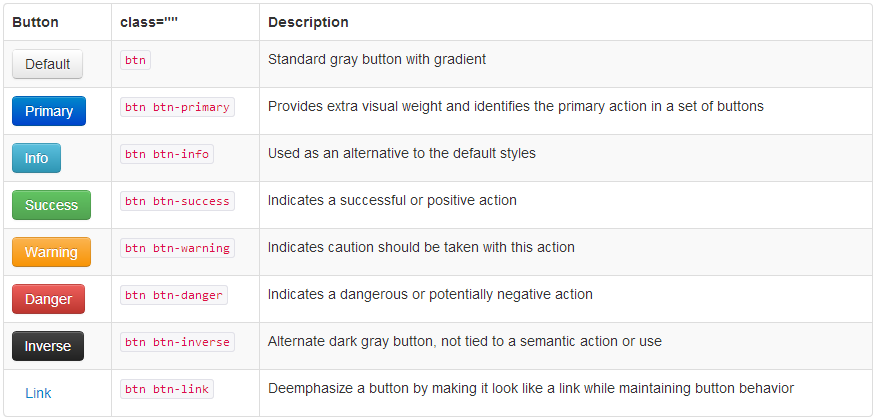
\includegraphics[width=\textwidth]{bootstrapbuttons}
\caption{Example of Twitter Bootstrap button types}
\end{figure}

\subsection{Icons}
Twitter Bootstrap comes with 140 sprite form icons, in both dark grey and white\footnote{Bootstrap icons: \url{http://twitter.github.com/bootstrap/base-css.html\#icons}} 

\newpage
At their site they feature some examples that can be used as a basis for development. We decided to base our web application design on this layout, as it suited our needs and was very close to our initial mockup
\begin{figure}[h!]
\label{bootstrapexample}
\centering
	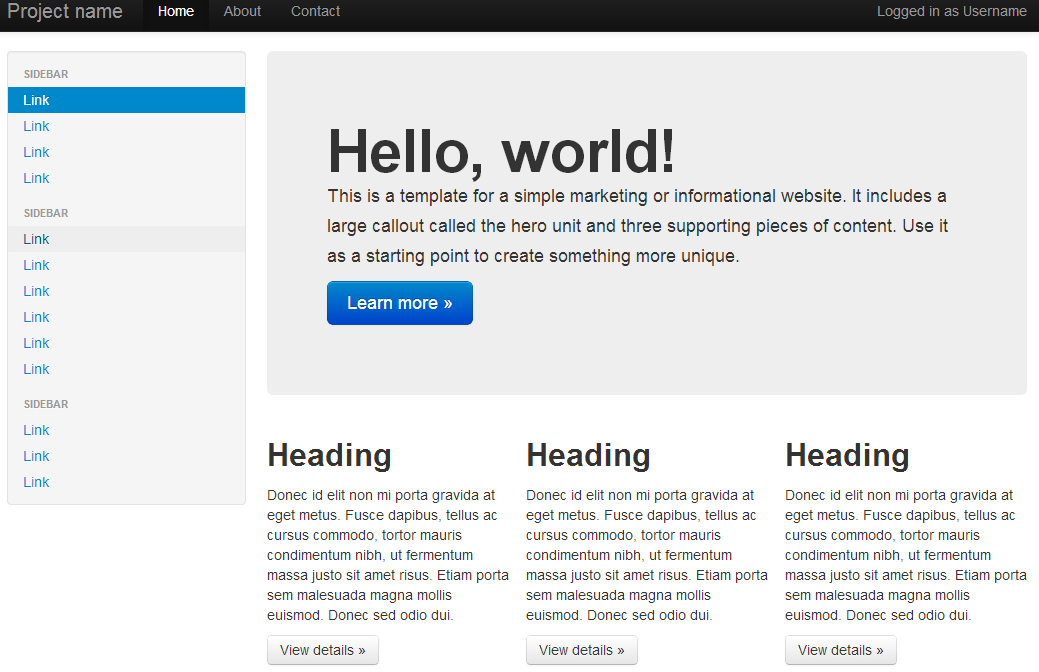
\includegraphics[width=\textwidth]{bootstrapexample}
\caption{Twitter bootstrap fluid layout with header and sidebar}
\end{figure}

Visiting the site on a mobile device with a smaller screen, the responsive fluid layout would optimize the page to look like this:
\begin{figure}[h!]
\label{bootstrapresponsive}
\centering
	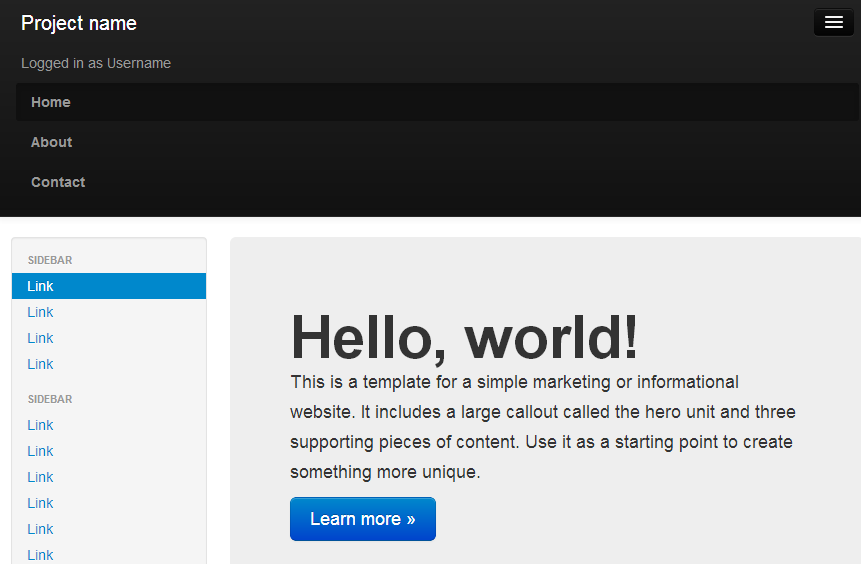
\includegraphics[width=\textwidth]{responsivemenuexample}
\caption{Twitter Bootstrap fluid layout with responsive menu and content}
\end{figure}
\newpage
And this is how our web-app looked after implementing bootstrap for a fully fluid and responsive web-application:
\begin{figure}[h!]
\label{teamscreen}
\centering
	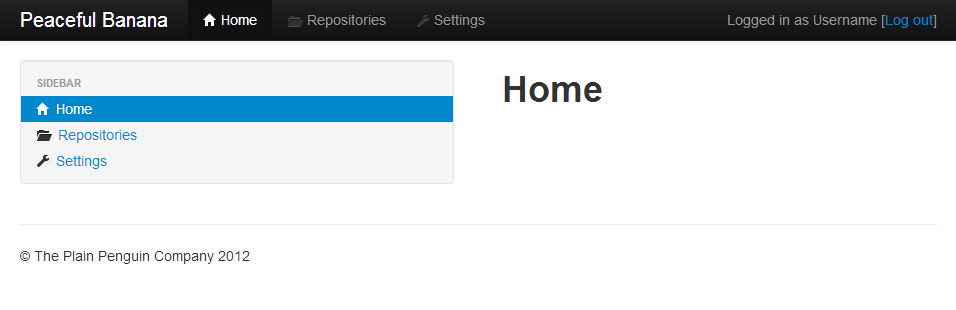
\includegraphics[width=\textwidth]{initial}
\caption{PeacefulBanana - Initial setup with Twitter Bootstrap}
\end{figure}

\section{PeacefulBanana Design}
After setting up and integrating the twitter bootstrap framework, the PeacefulBanana web-application was born, fully responsive and available on multiple platforms. This is how the final PeacefulBanana design looks like, it is based on the bootstrap example previously shown:
\begin{figure}[h!]
\label{finalhome}
\centering
	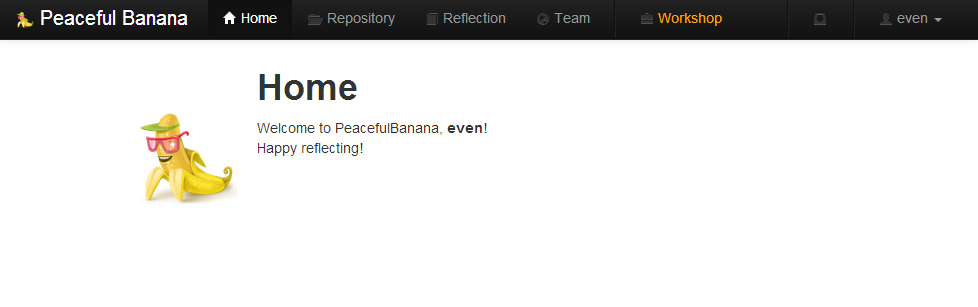
\includegraphics[width=\textwidth]{finalhome}
\caption{PeacefulBanana - Final home screen}
\end{figure}
The design is based on the Twitter Bootstrap framework and the principles of responsive web-design and a fluid layout. More specifically it is based on the fluid layout example\footnote{\url{http://twitter.github.com/bootstrap/examples/fluid.html}}. The PeacefulBanana layout features a navigation-menu on top with different tabs, leading to different content. Each of these tabs contain sidebars, which acts as submenus. The tool also integrates a user-menu, which is a dropdown with different actions that relates to the user, like settings. 

\subsection{Icons}
The PeacefulBanana tool makes extensive use of the icons included in Twitter Bootstrap, in order to further define what action you can expect from a tab. For example a home icon on the \textit{Home} tab, a globe on the \textit{Team} tab and a user icon on the \textit{User dropdown}.
\begin{figure}[h!]
\label{iconexample}
\centering
	
\includegraphics[width=\textwidth]{iconexample}
\caption{Example of Twitter Bootstrap/Glyphicons use in PeacefulBanana}
\end{figure}
